\section{Introduction}\label{sec:intro}
Cut cell meshes to solve hyperbolic problems 
are increasingly prevalent due to the ease 
of grid generation for complicated geometries \cite{}. 
However the {\em small cell} problem is still an active area of research, and
a completely satisfactory solution has not yet been found.
The small cell problem can be explained as follows: explicit
finite volume schemes typically need to take a time step 
that is proportional to the mesh width in order to satisfy a CFL constraint for
stability. However cut cells can have volumes that are arbitrarily
smaller than the regular cells that would otherwise determine the stable time
step. Special algorthms are needed to prevent this restriction.

The most commonly used stabilization algorithm is called flux
redistribution \cite{chern:colella,vof:colella}. The main idea is illustrated below in two space
dimensions, for ease of notation.
The essential idea is to compute the 
flux update for a cut cell $i,j$ with volume $V_{i,j} < V_{\mbox{\em full}}$,
\begin{eqnarray*}
V_{i,j} Q_{i,j} ^{n+1} & = V_{i,j} Q_{i,j}^n  +  \Delta t \, \Sigma_k F_k \cdot l_{k}\\
                   & = V_{i,j} Q_{i,j}^n  +  \delta  M 
\end{eqnarray*}
Here, $V_{\mbox{\em full}}$ is the volume of a full uncut cell.
Instead of using the entire amount of the update in cell ${i,j}$, 
the cut cell only uses a fraction $\eta$ of it.  If the fraction $\eta$
is proportional to the cell's volume
fraction $V_{i,j}/V_{\mbox{\em full}}$, the update should be stable. 
To maintain conservation, the rest of the update ($1-\eta)\delta M$
is given to the cell's neighbors.  
There are additional steps to make the distribution more robust and
accurate - see \cite{} for details.
Flux redistribution has already been implemented for three dimensional
calculations due to its simplicity. However it is only first order
accurate at the cut cells.

Cell merging \cite{} is most frequently the first idea people 
think of . It is conceptually simple, but 
we are not aware of any production codes that implement this in a fully
general, robust manner for complicated engineering geometries. 
The $h$-box method \cite{}
is a second order accurate method at the cut cells. It extends the 
domain of dependence for the fluxes around a small cell in a 
special way that maintains stability by means of a cancellation
property. It  has not been extended to
three dimensions due to its complexity. 

MORE OVERVIEW - the GEORGIA TECH
GUYS, the GERMAN GROUP, SANDRA IMPLICIT/EXPLICIT APPROACH, OTHERS?

Other approaches that have been proposed in the literature include
interpolation-based procedures, such as the mirror-cell method by Forrer
and Jeltsch \cite{article:FoJe98}, and a related ghost-fluid method by
Dadone and Grossman \cite{DadoneGrossman}.
There are also approaches based on finite difference schemes
\cite{SjogreenPetersson,MarcoBjorn}
and kinetic schemes \cite{Oksuzoglu:thesis,KeenKarni}.
However, since we are interested in methods
that preserve conservation we do not explore these alternatives further.

In this paper we propose a framework for a stabilization algorithm in
the spirit of flux redistribution (henceforth FRD). 
As with FRD, it is applied as a postprocessing
step, and is simple to implement. Cell updates on all cells are performed
in the usual way, followed by a postprocessing step based on the
conserved state variables, not on the fluxes.
Hence we call it {\em state redistribution} (SRD).

The simplest version is first order,
the use of a gradient makes it linearly exact, and the framework can be
extended to include higher order implementations as well. 
It is based on the following simple idea which we illustrate
here in one space dimension using the  first order upwind scheme.
We use the notation in  figure \ref{fig:modelProblem1}, which shows a
model problem with one
small cell with mesh width  $\alpha h, 0 < \alpha \leq 1$ in an
otherwise regular grid with mesh width $h$.

\begin{figure}
\begin{center}
%\vspace*{-.5in}
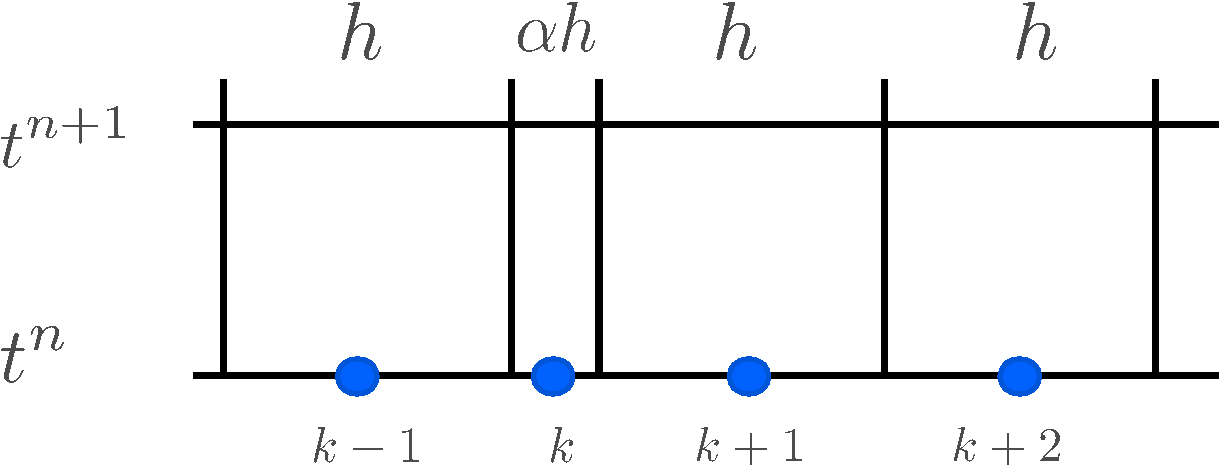
\includegraphics[height=1.3in]{figs/1dfig.pdf}
\caption{\sf Notation for model problem in one space dimension. The small
cell has size $\alpha h$ in a mesh with regular mesh width $h$.}
\label{fig:modelProblem1}
\end{center}
\end{figure}

To set the stage, notice that cell merging can
be rewritten as a postprocessing step.
To take one step to update a finite volume approximation to
$u_t + u_x = 0$ we do the following:
\begin{itemize}
\setlength\itemsep{.2in}
\item
{\bf Finite Volume Step}\\
Take the usual finite volume step with fixed, regular  $\Delta t$ on all cells 
including the small cell:
\begin{equation}
\bar{u}_j = u_j^n - \frac{\Delta t}{h_j} \; (f_{j+1/2} - f_{j-1/2} ), 
\quad \forall j.
\label{eqn:fvupdate}
\end{equation}

\item
{\bf {\em Temporarily} Create Merged Cell}\\
Temporarily create the {\em merged} cell $\overline{u_M}$ consisting of the small cell $u_j$ and one
or both of its neighbors so that it the merged cell is of sufficient
size (to be discussed later).  For simplicity here we will merge 
only with the neighbor on the right,
\begin{equation}
\widehat{u_M} =  \frac{ h_k \bar{u}_k + h_{k+1} \bar{u}_{k+1} } {h_k +
h_{k+1}} .
\label{eqn:mergestep}
\end{equation}

\item
{\bf Compute Merge Cell Gradient }\\
There are several ways to do this. 
Two simple possibilities are 
\begin{equation}
\nabla \widehat{u_M} = \frac{\bar{u}_{k+2} - \bar{u}_{k-1}} {x_{k+2}-x_{k-1}}
\label{eqn:gradLim1}
\end{equation}
which does not use the merged cell,
or
\begin{equation}
\nabla \widehat{u_M} = \frac{\bar{u}_{k+2} - \widehat{u_{M}}} {x_{k+2}-x_{M}}
\label{eqn:gradLim2}
\end{equation}
which uses the merged cell, and $x_M$ is the centroid of the merged
cell.
The choice of gradient stencil will be studied later in section \ref{sec:srdAlg}.

%Other more accurate alternatives exist, not all of which are stable.
%It would be better to use smaller stencils, perhaps including $u_{k+1}$
%or $\overline{u_M}$ itself.

\item
{\bf Redistribute Merged State to Cells Comprising Merged cell }\\
Replace the provisional values computed in the cells comprising the
merged cell with the merged solution reconstructed to the cell
centroids:
\begin{equation}
\begin{split}
u_k^{n+1} &= \widehat{u_M} +  (x_k - x_M) \nabla \widehat{u_M}\\
u_{k+1}^{n+1} &= \widehat{u_M} +  (x_{k+1} - x_M) \nabla \widehat{u_M}
\end{split}
\end{equation}
\end{itemize}
This method is clearly linearity preserving if all gradients are
computed accurately enough to preserve a linear function.  
It is conservative since the mass of the merged cell equals the mass of
the two cells comprising it, and the linear function through the
centroid also has the same amount of total mass.

When written in one-step form instead of as a post-processing step, 
it is seen to be closely related to cell merging. 
In the first order case without gradient, the above gives
\begin{equation}
u_k^{n+1} = u_{k+1}^{n+1} = \widehat{u_M}^{n+1} 
\end{equation}
Pluging in the updates for $\widehat{u_M}$ we get
\begin{equation}
\widehat{u_M}^{n+1} = \widehat{u_M}^n - 
\frac{\Delta t}{h_k + h_{k+1}} (f_{k+3/2} - f_{k-1/2})
\end{equation}
Recognizing that $h_k+h_{k+1}$ is the merged cell volume makes this
clear.
By using a higher than linear polynomial and
including more neighbors in the
redistribution (on top of a more accurate scheme for the entire grid),
we have a path to higher order accuracy.
%By including gradients it provides a path to higher dimensions, possibly 
%overlapping neighborhoods. 

The choice of merging neighborhoods and gradients is what makes up the
specifics of SRD in two space dimensions. Furthermore, it can happen
that a cell has more than one neighborhood with
which it should merge. This is what often causes complications in cell
merging algorithms. In SRD, we will simply use all such values appropriately
weighted.

In the next section  we first review the finite volume schemes to which SRD will
be applied.
The SRD algorithm in two space dimensions will be presented in section
\ref{sec:srdAlg}.
For simplicity we present the second order accurate version first.
The more general higher order extension is described in 
section \ref{sec:ho}.
Some theoretical results using one-dimensional model problems are in
section \ref{sec:theory}. 
Section \ref{sec:compResults} shows computational results for both smooth
problems and shocked flow for both linear advection and the Euler equations.  We conclude in section \ref{sec:conc}.
